\documentclass[a4paper,11pt]{article}
\usepackage[a4paper,total={18cm, 24cm}]{geometry}
\usepackage[parfill]{parskip}
\usepackage[utf8]{inputenc}
\usepackage[T1]{fontenc}
\usepackage{fancyhdr}
\usepackage[ddmmyyyy]{datetime}
\usepackage{graphicx}
\usepackage{subcaption}

\pagestyle{fancy}
\fancyhf{}
\lhead{\today}
\chead{Deep Learning - Double Descent}
\rhead{Jakub Rada}

\begin{document}
\section{Assignment introduction}
This is a report for the first assignment regarding Double Descent.
I implemented the learning of the linear layer as discussed during the tutorial class
\[
    \theta = (\Phi^T \Phi + \lambda I)^{-1}\Phi^Ty
\]
, where $\Phi$ is the data matrix $N\times(D+1)$ and $\lambda = 10^{-6}$.

The neural network then computes the scores by first lifting the dimension of input data (prepared in the template) and computing a linear layer with the computed weights $\theta = (w, b)$ as
\[
    s = w^t \phi + b
\]

\section{Task 1}
\subsection{Decision boundary}
First part of task 1 was to fix training size to $40$ and try different values of $D$ for training to see the learned decision boundaries.
I tried many values rangin from $10$ to $1000$ and the results are shown in the figures below.

\begin{figure}[ht]
    \begin{subfigure}[b]{0.3\textwidth}
        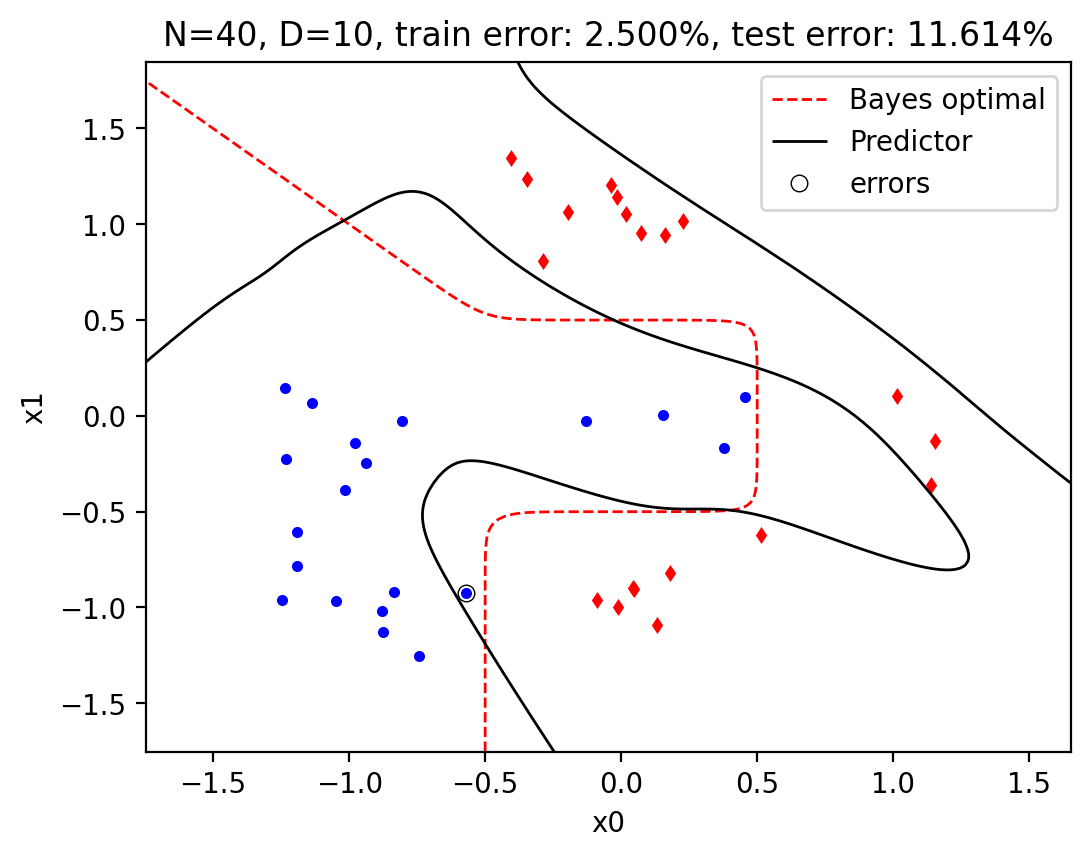
\includegraphics[width=\textwidth]{../boundary/10.png}
    \end{subfigure}
    \hfill
    \begin{subfigure}[b]{0.3\textwidth}
        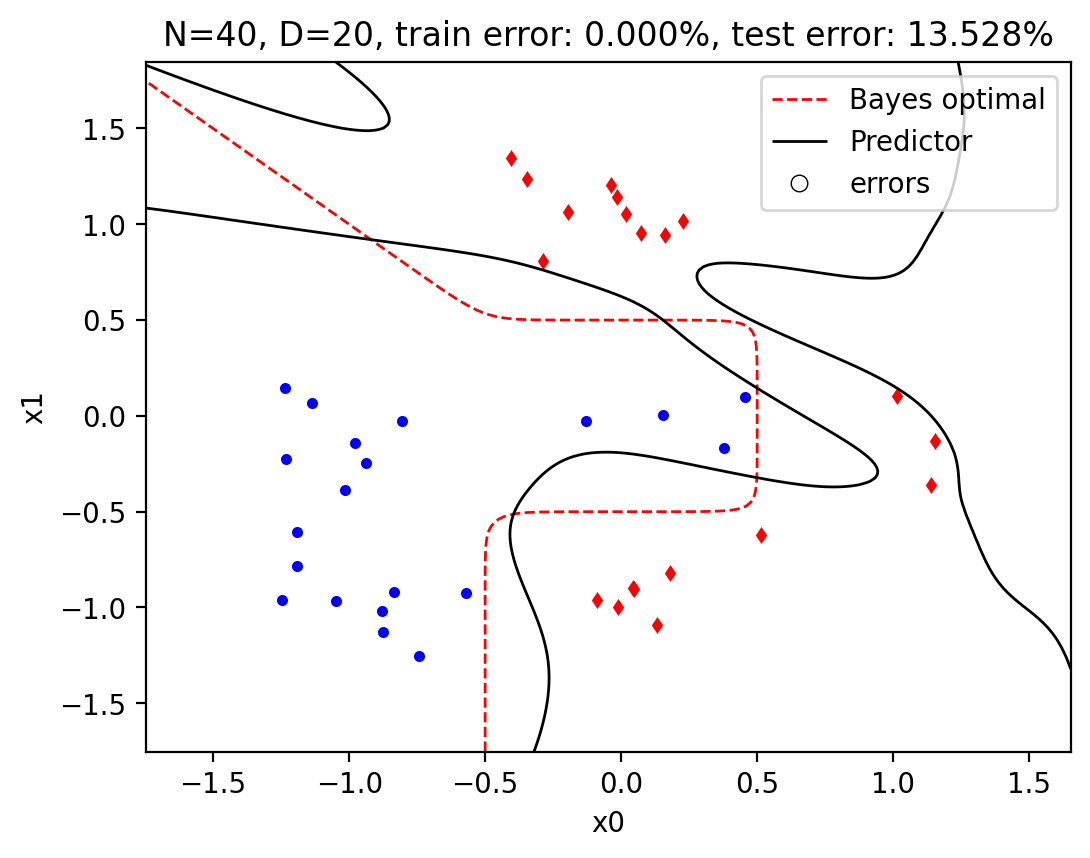
\includegraphics[width=\textwidth]{../boundary/20.png}
    \end{subfigure}
    \hfill
    \begin{subfigure}[b]{0.3\textwidth}
        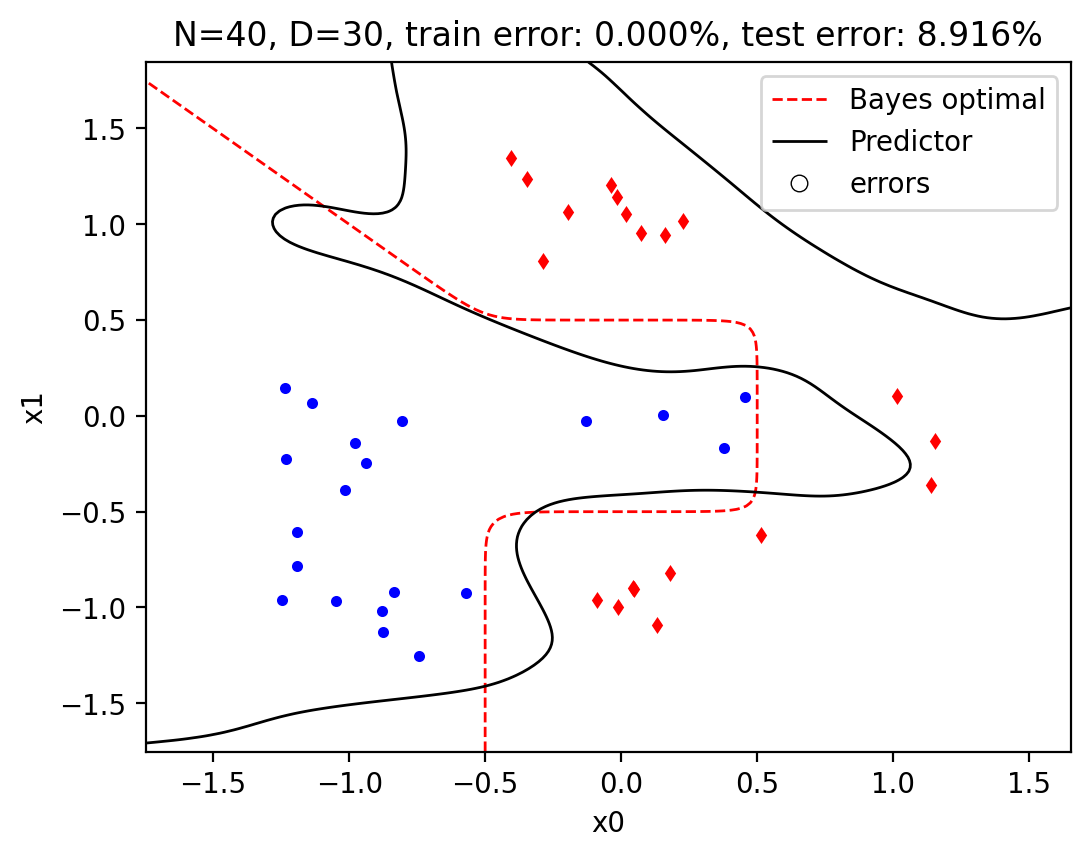
\includegraphics[width=\textwidth]{../boundary/30.png}
    \end{subfigure}
    \begin{subfigure}[b]{0.3\textwidth}
        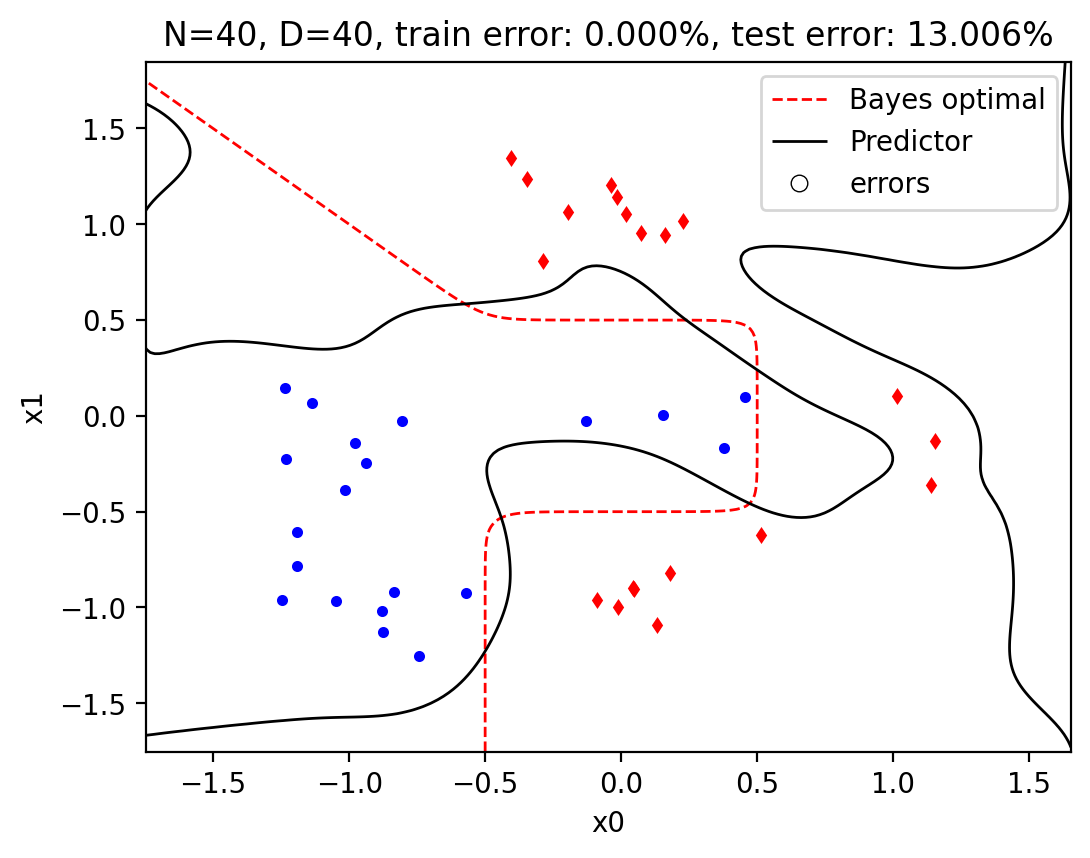
\includegraphics[width=\textwidth]{../boundary/40.png}
    \end{subfigure}
    \hfill
    \begin{subfigure}[b]{0.3\textwidth}
        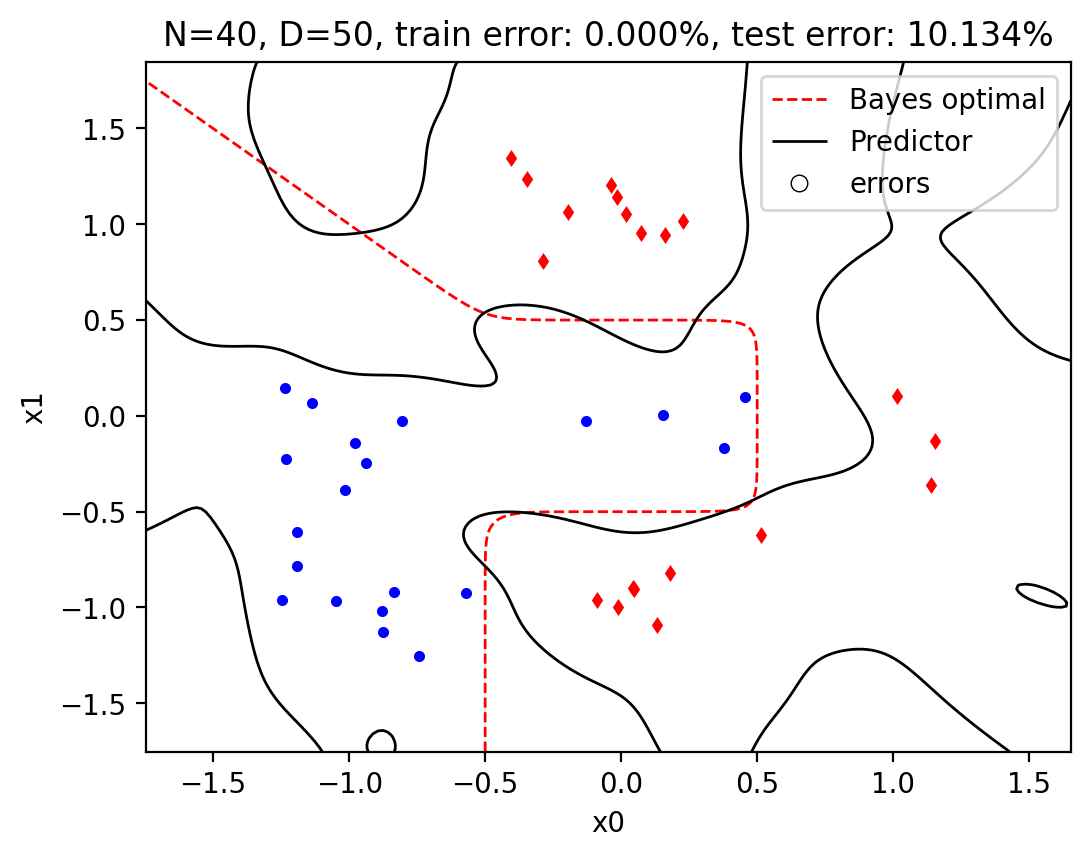
\includegraphics[width=\textwidth]{../boundary/50.png}
    \end{subfigure}
    \hfill
    \begin{subfigure}[b]{0.3\textwidth}
        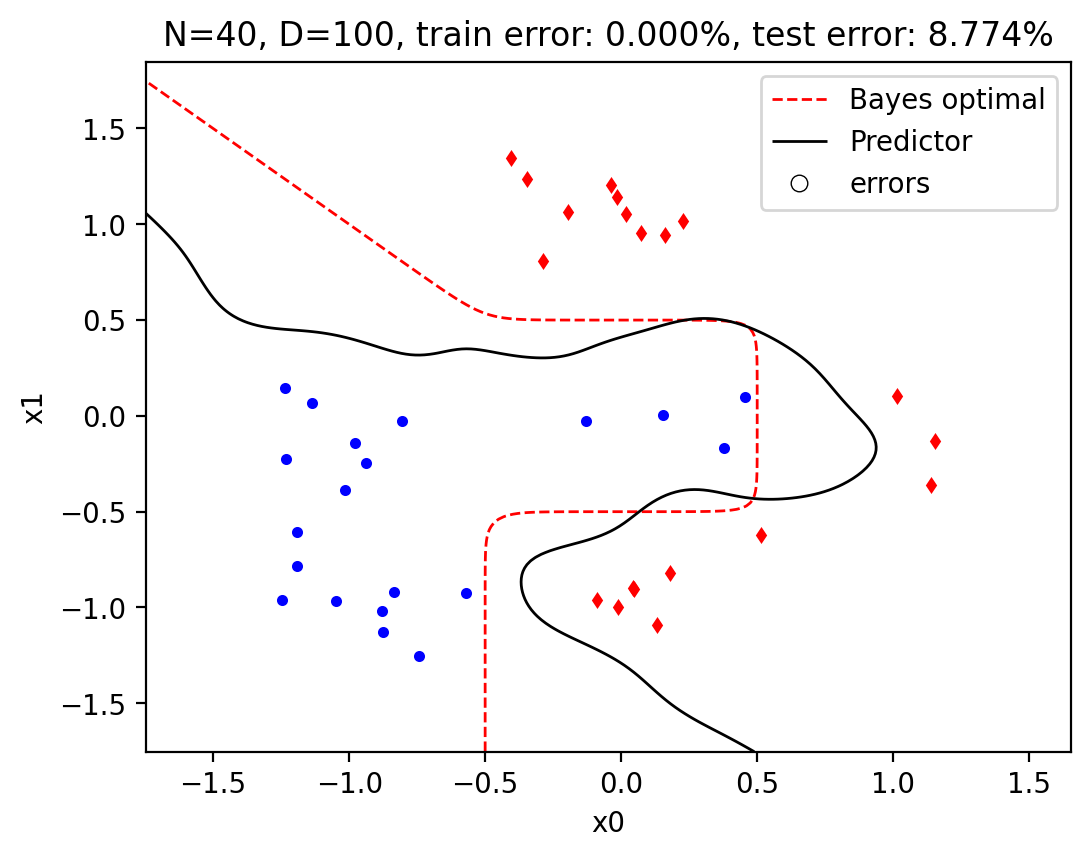
\includegraphics[width=\textwidth]{../boundary/100.png}
    \end{subfigure}
    \begin{subfigure}[b]{0.3\textwidth}
        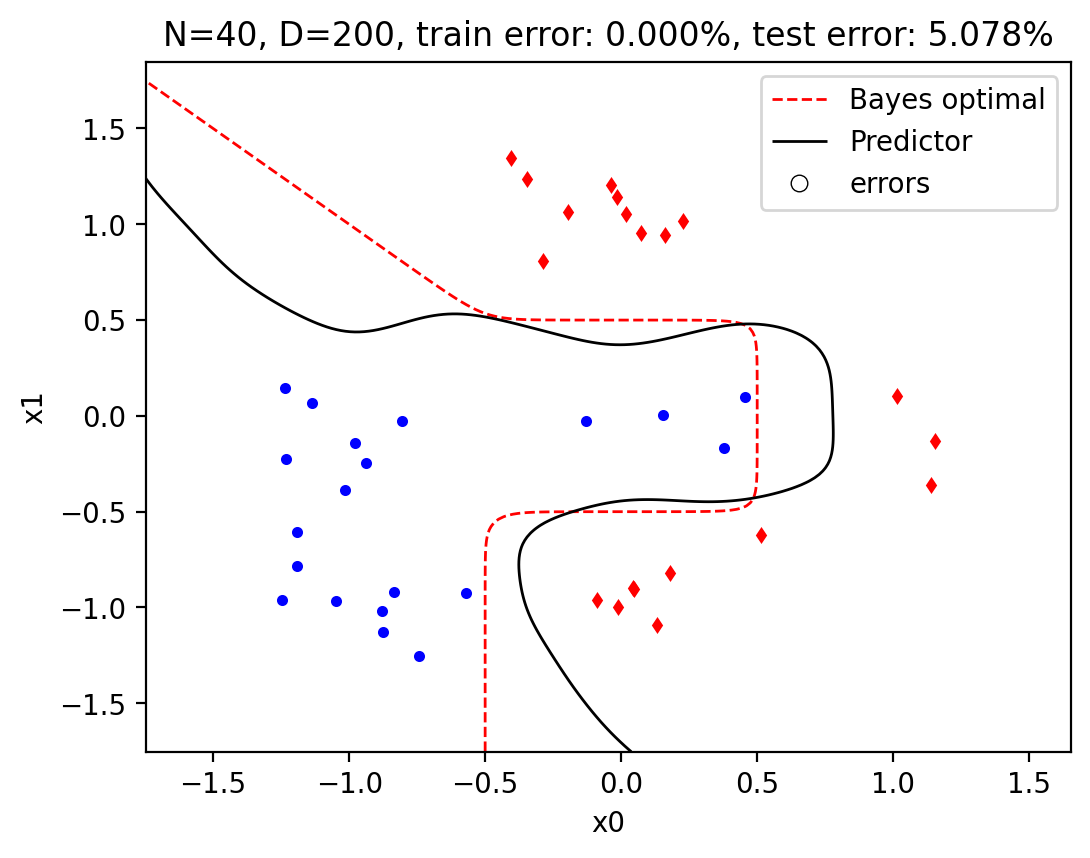
\includegraphics[width=\textwidth]{../boundary/200.png}
    \end{subfigure}
    \hfill
    \begin{subfigure}[b]{0.3\textwidth}
        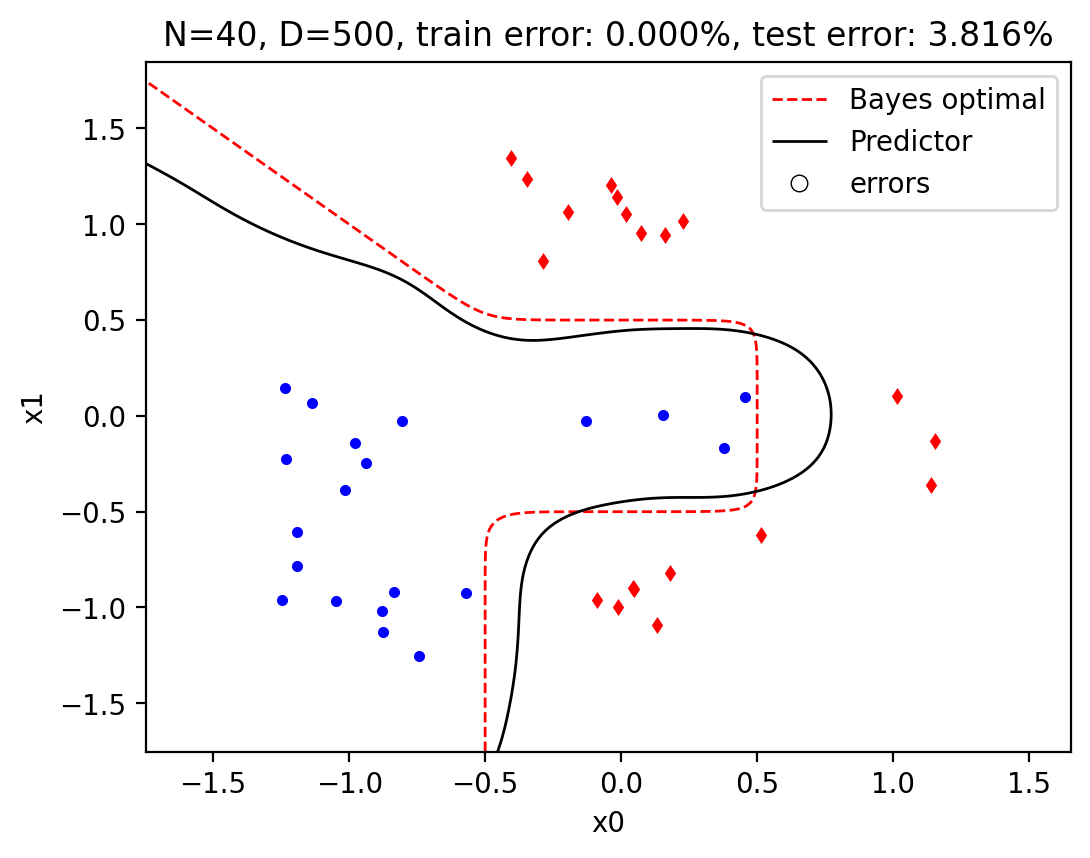
\includegraphics[width=\textwidth]{../boundary/500.png}
    \end{subfigure}
    \hfill
    \begin{subfigure}[b]{0.3\textwidth}
        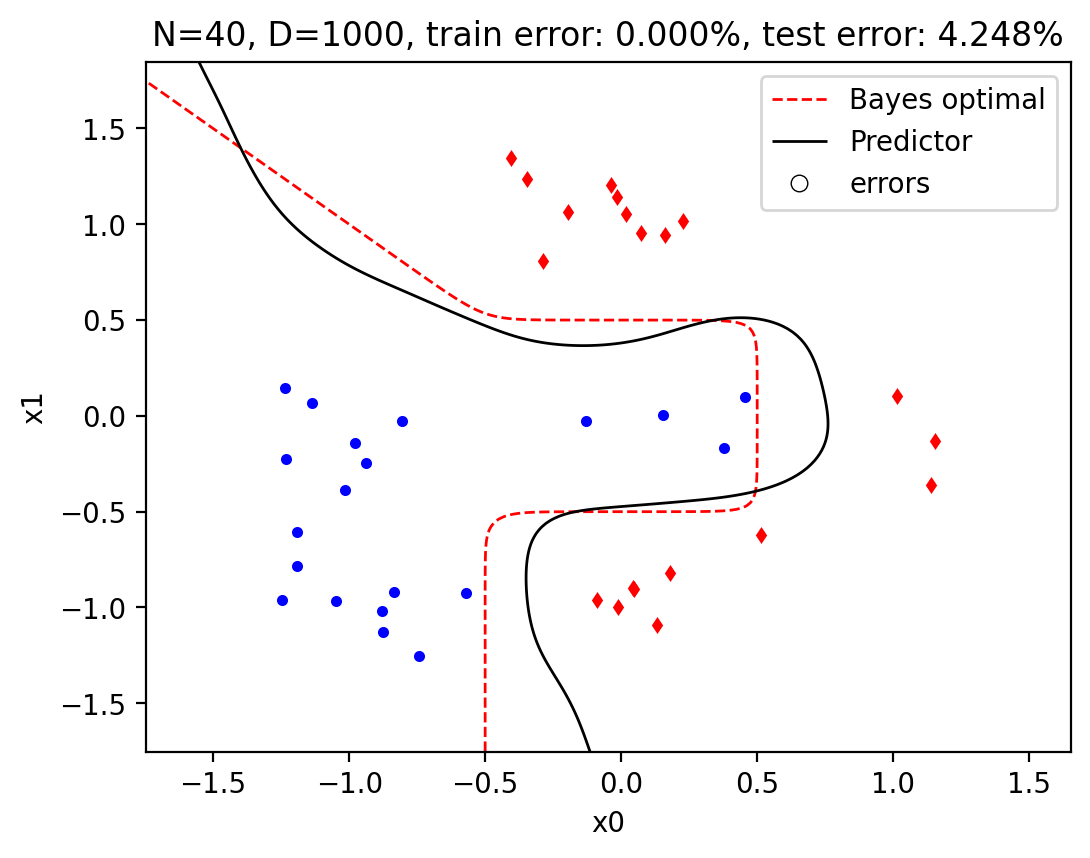
\includegraphics[width=\textwidth]{../boundary/1000.png}
    \end{subfigure}
    \caption{Decision boundaries for different hidden dimensions $D$}
\end{figure}

Every chart contains the number of training samples $N$, the hidden dimension $D$ and the training error and test error values.

By visual comparison, we can confirm the idea mentioned in the assignment, that the complexity of the decision boundary increases with hidden dimension up to around 40 (50 in my case) and then it decreases to a smooth line around the optimal bayes decision boundary.
The lowest test error is actually achieved for $D=500$.
This might be caused by the big difference in the sizes of training and test sets.
The network was trained on 40 samples and tested on 50000 samples.

\subsection{Influence of training set size}
Second part of task 1 was to fix the hidden dimension to $D=40$ and try different sizes of the training set $N=2,4,\dots,200$ to observe test error and test loss.
The loss was computed as \textit{Mean Square Error}
\[
    L = \frac{1}{N}\sum_{i=1}^{N}||y_i - s_i||^2
\].
The experiments for each $n \in N$ were repeated 100 trials and the resulting errors and losses were averaged.
The test set of size $50000$ was generated for each $n \in N$ but the training set and random lifting was generated for every trial independently.

The results are shown in the following figures.

\begin{figure}[ht]
    \centering
    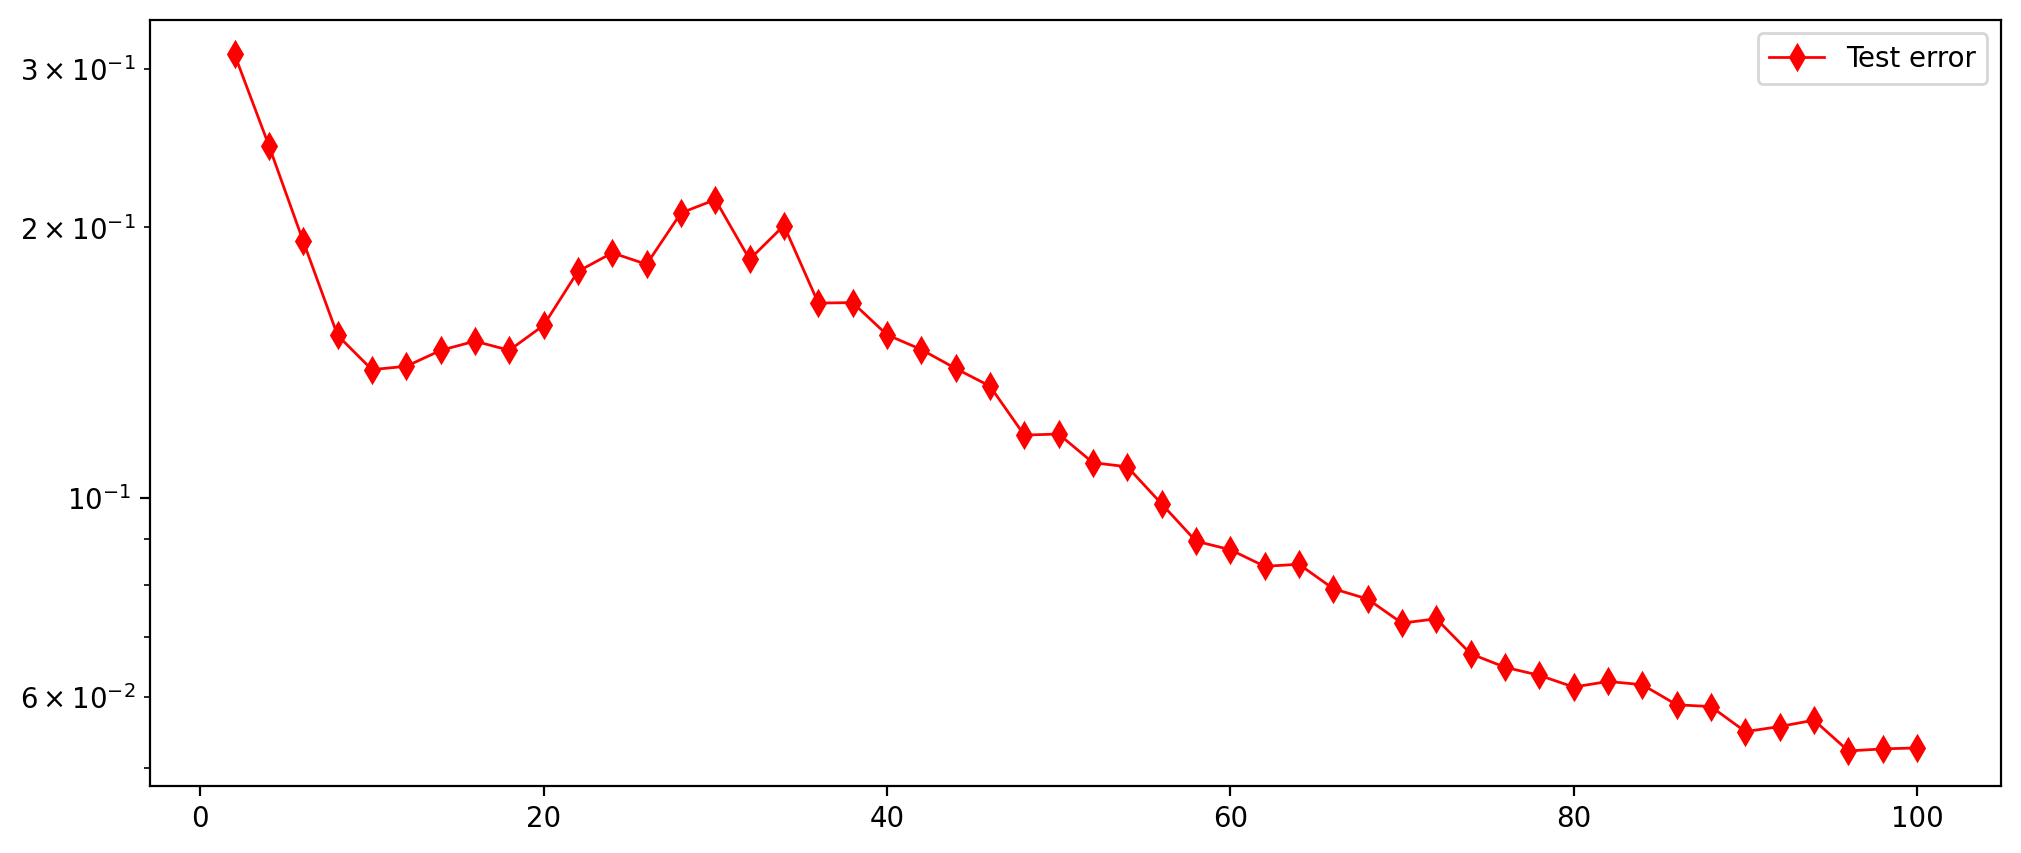
\includegraphics[width=0.8\textwidth]{../training_size/test_error.png}
    \caption{Test error for $n \in \{2, 4, 6, \dots, 100\}$}
\end{figure}

\begin{figure}[ht]
    \centering
    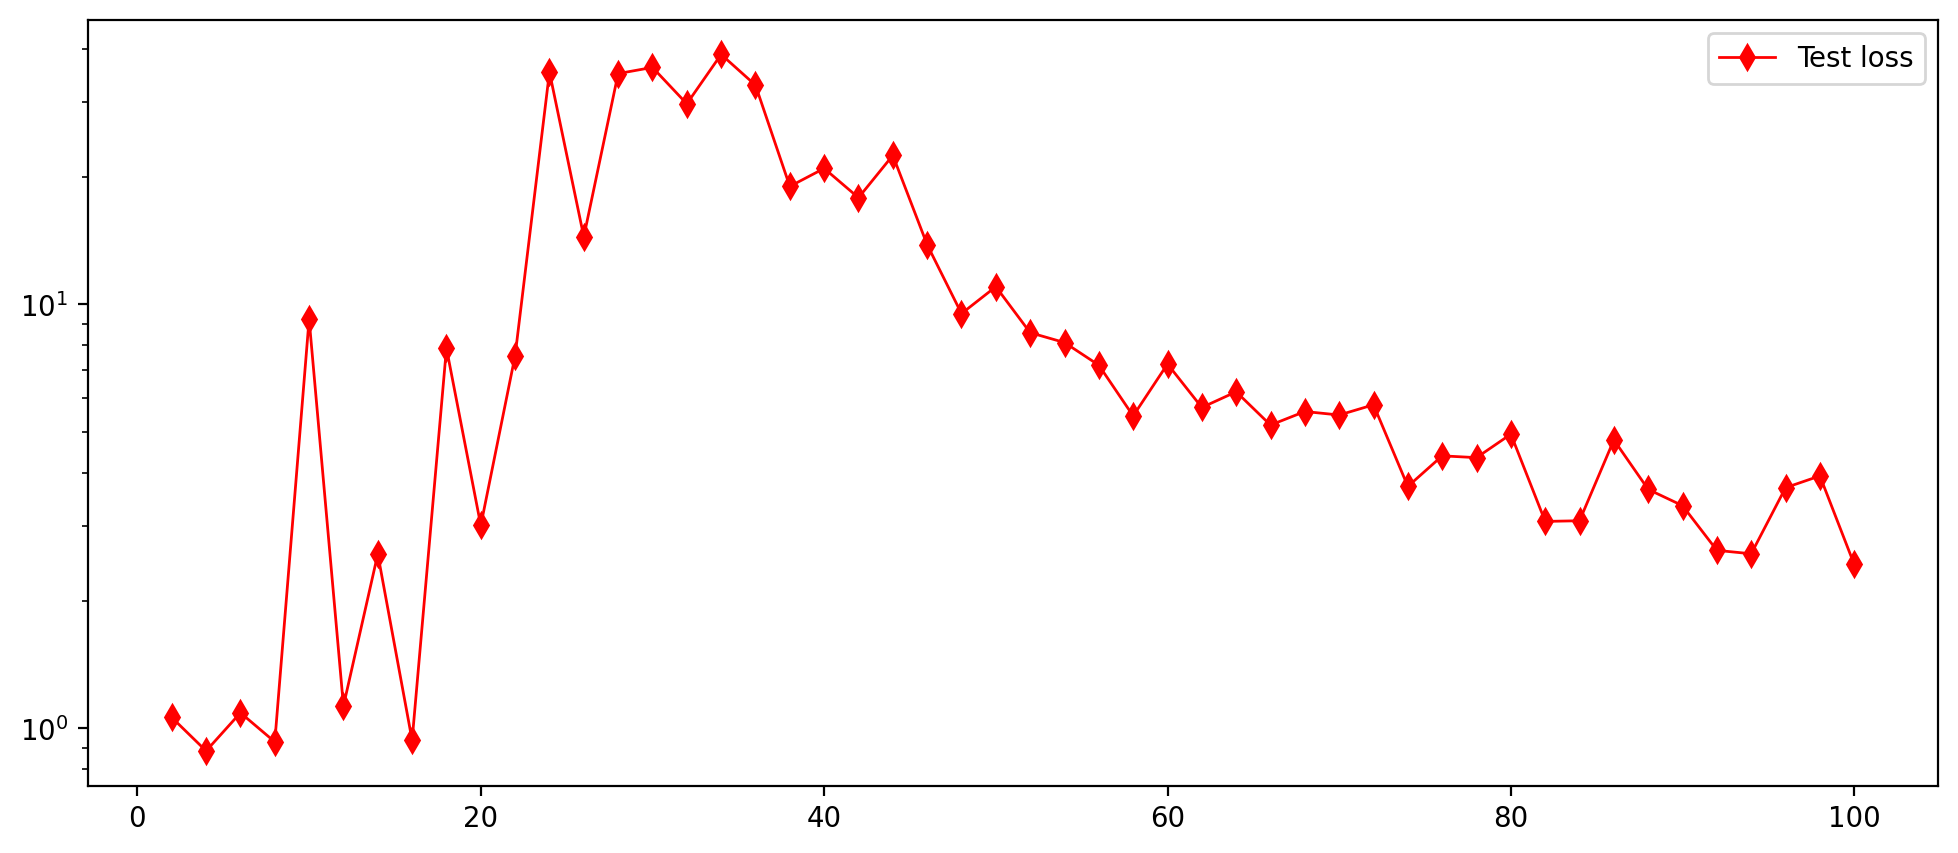
\includegraphics[width=0.8\textwidth]{../training_size/test_loss.png}
    \caption{Test MSE loss for $n \in \{2, 4, 6, \dots, 100\}$}
\end{figure}

In the charts we can see the double descent phenomenon. Test error starts to raise somewhere around 20 and continues to grow until around 40.
Then, it starts to decrease again.

From this plot it seems that simply more data yields better results.
However, we would have to test it for varying sizes of hidden dimension $D$ to confirm this.
The tendencies could be similar but the values where the error starts to decrease again can be different.

\section{Task 2}
In the last experiment we fix the training set size to $N=40$ and change the hidden dimension size $D=1,10,20,\dots,200$.
This experiment should confirm the same phenomenon as in previous task but now we study both training and test errors and losses.

The experiment was conducted in the same setting as the one before.
For each value of $d \in D$ we repeated the experiment 100 times and averaged the resulting errors and losses.
The test set was regenerated for each $d \in D$ but the training set and random lifting was generated for every trial at random.

\begin{figure}[ht]
    \centering
    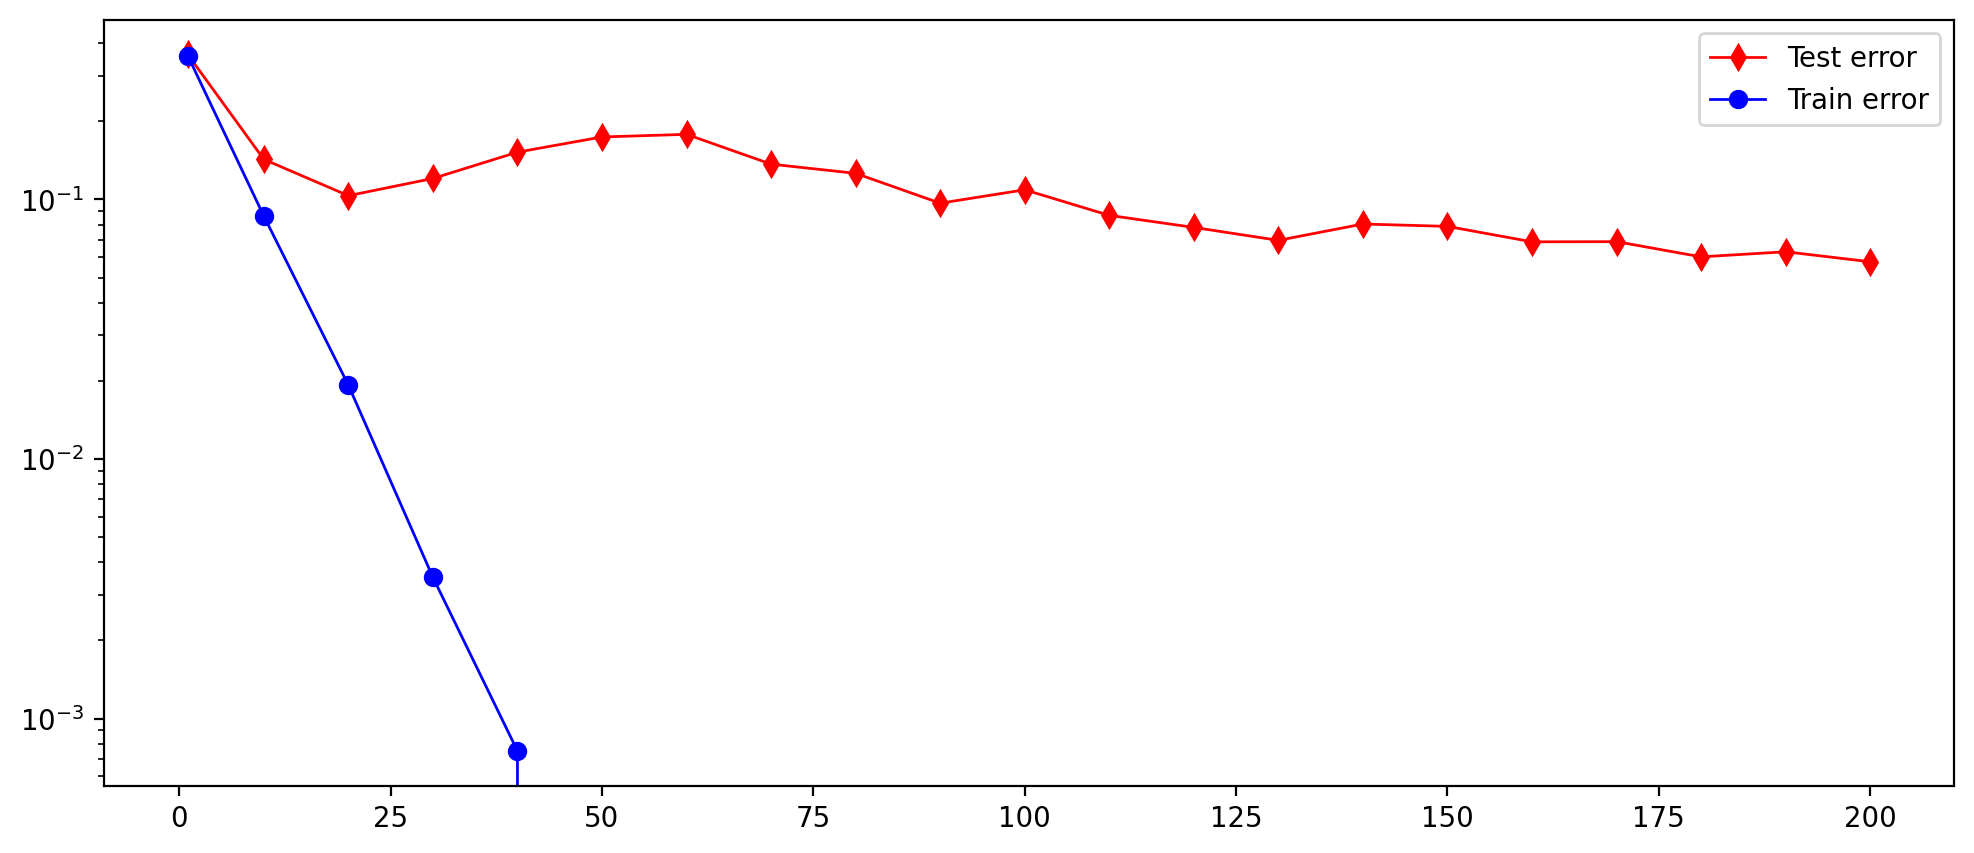
\includegraphics[width=0.8\textwidth]{../hidden_size/errors.png}
    \caption{Errors for $d \in \{1, 10, 20, \dots, 200\}$}
\end{figure}

\begin{figure}[ht]
    \centering
    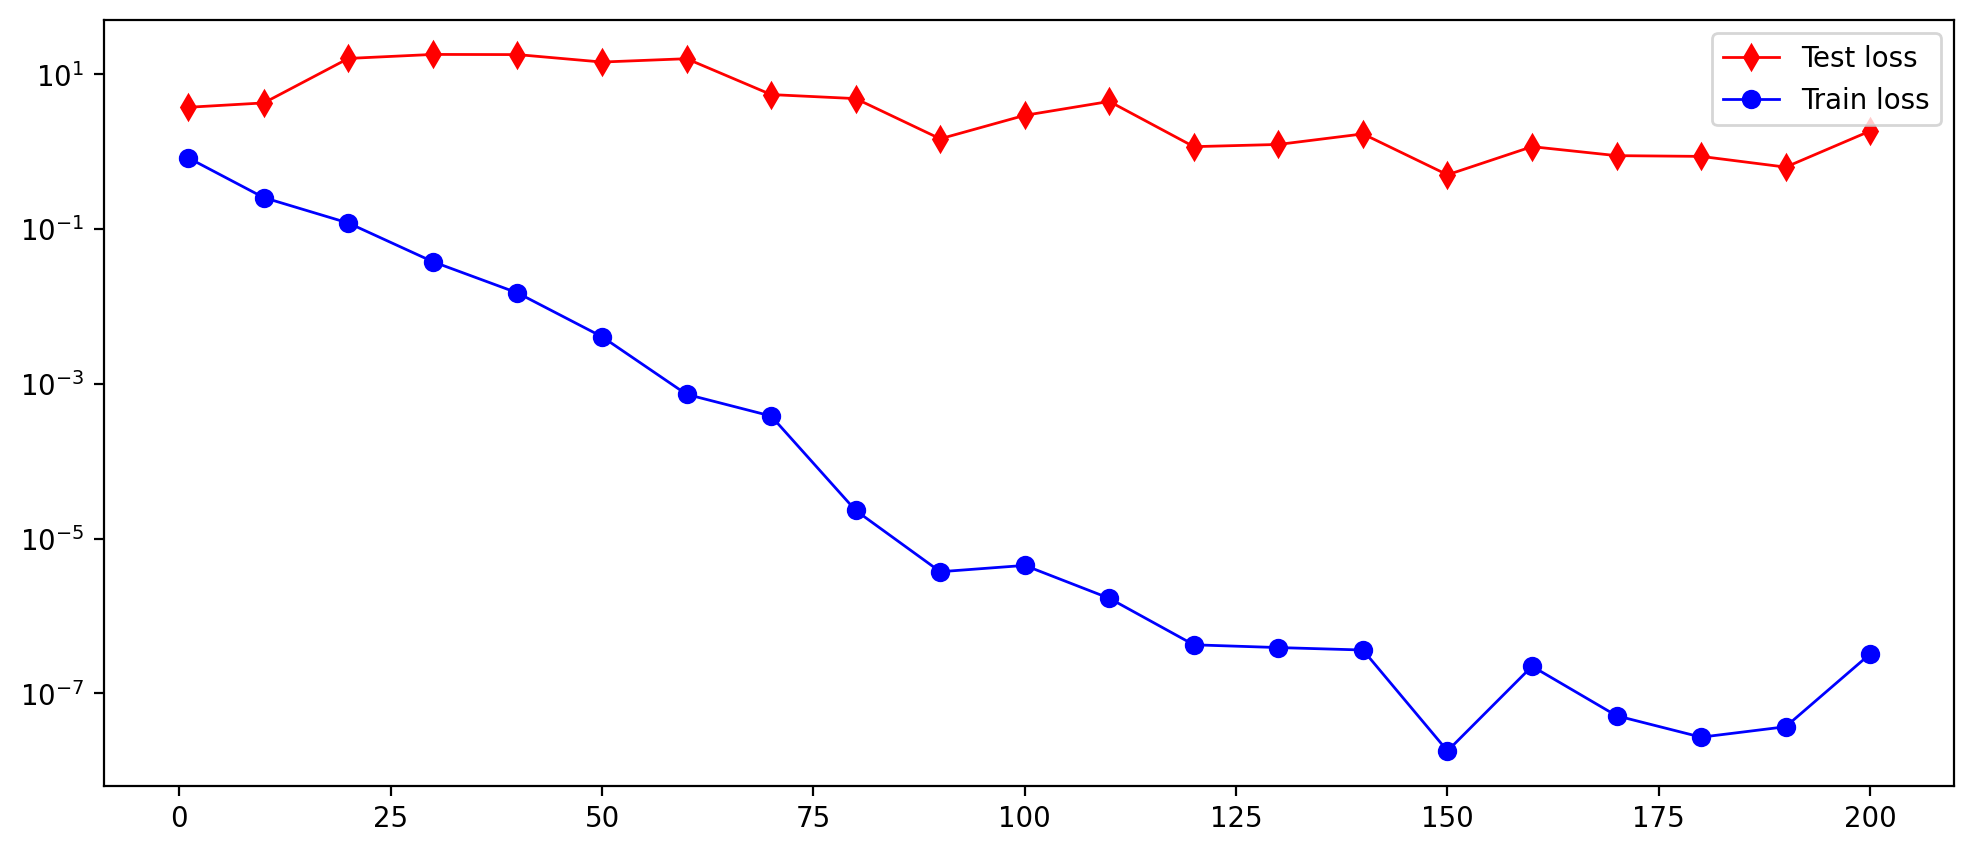
\includegraphics[width=0.8\textwidth]{../hidden_size/losses.png}
    \caption{MSE losses for $d \in \{1, 10, 20, \dots, 200\}$}
\end{figure}

From the graphs we can see that the same phenomenon occurs as in the previous task.
It is especially visible in the error chart, where we can see a rise of values around $d=50$.
Note that the scale of the $y$ axis is logarithmic, thus the rise in values is much bigger that what it looks like at first sight.
It is interesting to notice that the training error only decreases and also much more quickly implying that increasing size of the linear layer helps significantly for training.
However, it does not necessarily mean better generalization as seen by the bump in test error.

\section{Discussion}
As described in the paper linked on the webpage, this phenomenon is observed not only in such simple models as the one in this task but also in CNNs, DNNs and Transformers that are used in applications today.
According to the paper, we are not sure why this happens but we observe it consistently in different situations.
The size of the model has an impact, also the number of training samples has an impact on the so-called \textit{interpolation threshold}.
This threshold also influences the peak in test error.

I don't have a solid opinion on why it occurs.
I imagine that for every dataset there is a network that fits it just right but cannot fit anything more and this causes the increase when we add more data.
In this scenario, the overparametrization would work as kind of spreading the learned information across many more weights and thus leaving some "space" for generalization.
But I don't have any arguments for this, it's just an intuitive idea.

\end{document}
